% PGFPlots bar chart - Baseline Convergence by Technique
% Include in main document with % PGFPlots bar chart - Baseline Convergence by Technique
% Include in main document with % PGFPlots bar chart - Baseline Convergence by Technique
% Include in main document with % PGFPlots bar chart - Baseline Convergence by Technique
% Include in main document with \input{figures/convergence-chart.tex}

\begin{figure}[t]
\centering
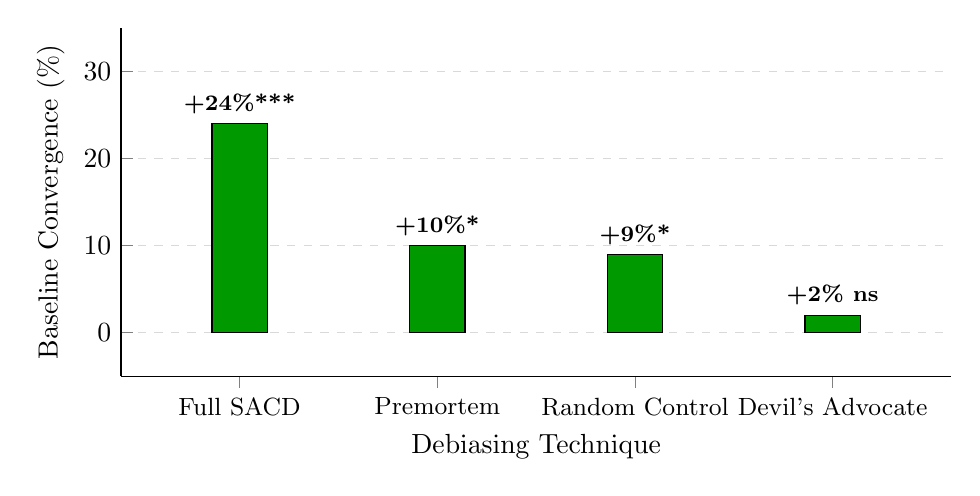
\begin{tikzpicture}
\begin{axis}[
    ybar,
    bar width=20pt,
    width=\columnwidth,
    height=6cm,
    ylabel={Baseline Convergence (\%)},
    xlabel={Debiasing Technique},
    ymin=-5,
    ymax=35,
    xtick=data,
    symbolic x coords={Full SACD, Premortem, Random Control, Devil's Advocate},
    xticklabel style={font=\small},
    nodes near coords,
    nodes near coords align={vertical},
    every node near coord/.append style={font=\footnotesize\bfseries},
    point meta=explicit symbolic,
    enlarge x limits=0.2,
    axis lines*=left,
    ymajorgrids=true,
    grid style={dashed,gray!30},
]
\addplot[fill=green!60!black, draw=black] coordinates {
    (Full SACD, 24) [+24\%***]
    (Premortem, 10) [+10\%*]
    (Random Control, 9) [+9\%*]
    (Devil's Advocate, 2) [+2\% ns]
};
\end{axis}
\end{tikzpicture}
\caption{Baseline convergence by debiasing technique. Positive values indicate the technique moves judgments toward the model's unprompted baseline. Full SACD shows strongest convergence (+24\%, $p<0.001$), significantly outperforming the Random Control (+9\%), demonstrating that iterative self-critique provides genuine debiasing beyond simple conversation length effects. *** $p<0.001$, * $p<0.05$, ns = not significant.}
\label{fig:convergence}
\end{figure}


\begin{figure}[t]
\centering
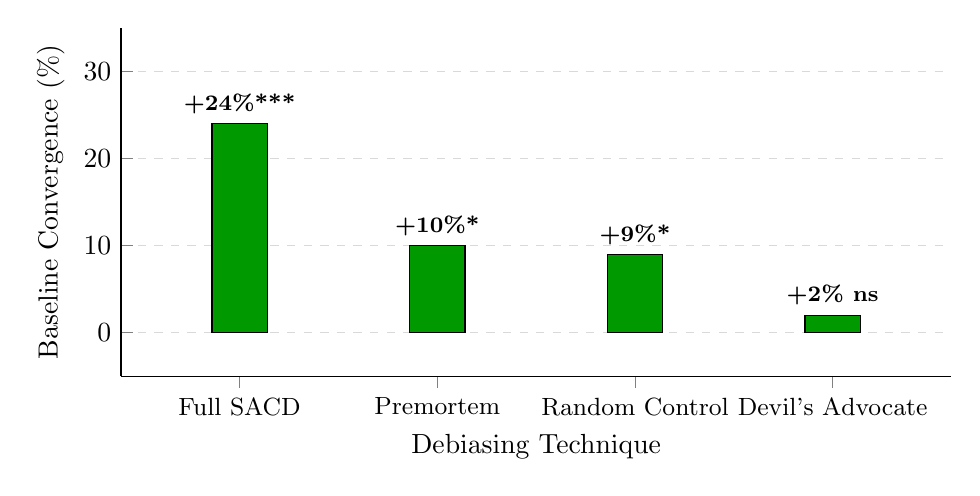
\begin{tikzpicture}
\begin{axis}[
    ybar,
    bar width=20pt,
    width=\columnwidth,
    height=6cm,
    ylabel={Baseline Convergence (\%)},
    xlabel={Debiasing Technique},
    ymin=-5,
    ymax=35,
    xtick=data,
    symbolic x coords={Full SACD, Premortem, Random Control, Devil's Advocate},
    xticklabel style={font=\small},
    nodes near coords,
    nodes near coords align={vertical},
    every node near coord/.append style={font=\footnotesize\bfseries},
    point meta=explicit symbolic,
    enlarge x limits=0.2,
    axis lines*=left,
    ymajorgrids=true,
    grid style={dashed,gray!30},
]
\addplot[fill=green!60!black, draw=black] coordinates {
    (Full SACD, 24) [+24\%***]
    (Premortem, 10) [+10\%*]
    (Random Control, 9) [+9\%*]
    (Devil's Advocate, 2) [+2\% ns]
};
\end{axis}
\end{tikzpicture}
\caption{Baseline convergence by debiasing technique. Positive values indicate the technique moves judgments toward the model's unprompted baseline. Full SACD shows strongest convergence (+24\%, $p<0.001$), significantly outperforming the Random Control (+9\%), demonstrating that iterative self-critique provides genuine debiasing beyond simple conversation length effects. *** $p<0.001$, * $p<0.05$, ns = not significant.}
\label{fig:convergence}
\end{figure}


\begin{figure}[t]
\centering
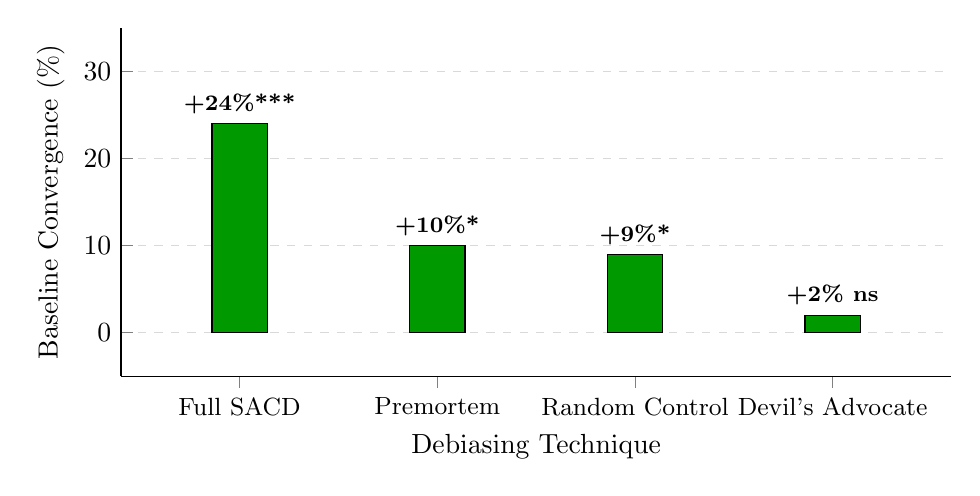
\begin{tikzpicture}
\begin{axis}[
    ybar,
    bar width=20pt,
    width=\columnwidth,
    height=6cm,
    ylabel={Baseline Convergence (\%)},
    xlabel={Debiasing Technique},
    ymin=-5,
    ymax=35,
    xtick=data,
    symbolic x coords={Full SACD, Premortem, Random Control, Devil's Advocate},
    xticklabel style={font=\small},
    nodes near coords,
    nodes near coords align={vertical},
    every node near coord/.append style={font=\footnotesize\bfseries},
    point meta=explicit symbolic,
    enlarge x limits=0.2,
    axis lines*=left,
    ymajorgrids=true,
    grid style={dashed,gray!30},
]
\addplot[fill=green!60!black, draw=black] coordinates {
    (Full SACD, 24) [+24\%***]
    (Premortem, 10) [+10\%*]
    (Random Control, 9) [+9\%*]
    (Devil's Advocate, 2) [+2\% ns]
};
\end{axis}
\end{tikzpicture}
\caption{Baseline convergence by debiasing technique. Positive values indicate the technique moves judgments toward the model's unprompted baseline. Full SACD shows strongest convergence (+24\%, $p<0.001$), significantly outperforming the Random Control (+9\%), demonstrating that iterative self-critique provides genuine debiasing beyond simple conversation length effects. *** $p<0.001$, * $p<0.05$, ns = not significant.}
\label{fig:convergence}
\end{figure}


\begin{figure}[t]
\centering
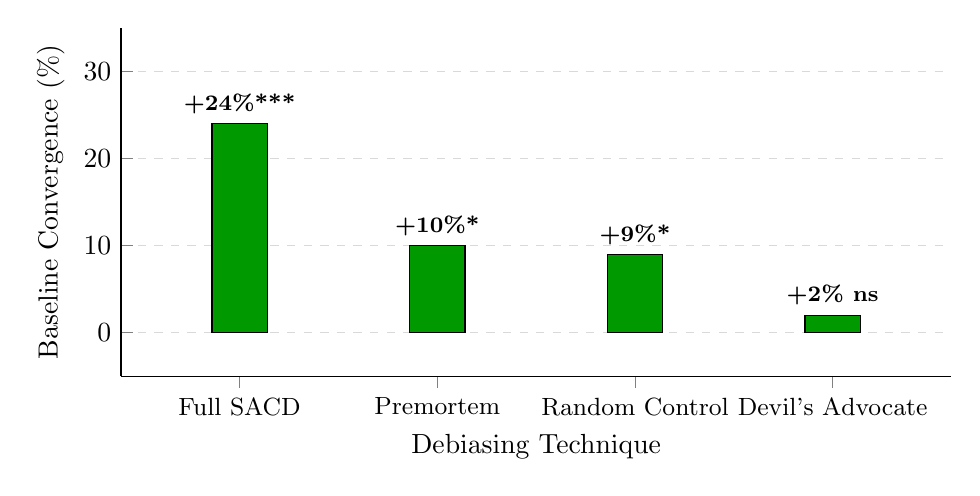
\begin{tikzpicture}
\begin{axis}[
    ybar,
    bar width=20pt,
    width=\columnwidth,
    height=6cm,
    ylabel={Baseline Convergence (\%)},
    xlabel={Debiasing Technique},
    ymin=-5,
    ymax=35,
    xtick=data,
    symbolic x coords={Full SACD, Premortem, Random Control, Devil's Advocate},
    xticklabel style={font=\small},
    nodes near coords,
    nodes near coords align={vertical},
    every node near coord/.append style={font=\footnotesize\bfseries},
    point meta=explicit symbolic,
    enlarge x limits=0.2,
    axis lines*=left,
    ymajorgrids=true,
    grid style={dashed,gray!30},
]
\addplot[fill=green!60!black, draw=black] coordinates {
    (Full SACD, 24) [+24\%***]
    (Premortem, 10) [+10\%*]
    (Random Control, 9) [+9\%*]
    (Devil's Advocate, 2) [+2\% ns]
};
\end{axis}
\end{tikzpicture}
\caption{Baseline convergence by debiasing technique. Positive values indicate the technique moves judgments toward the model's unprompted baseline. Full SACD shows strongest convergence (+24\%, $p<0.001$), significantly outperforming the Random Control (+9\%), demonstrating that iterative self-critique provides genuine debiasing beyond simple conversation length effects. *** $p<0.001$, * $p<0.05$, ns = not significant.}
\label{fig:convergence}
\end{figure}
